\begin{justifying}
 \title{
   \begin{center}
    \normalsize CAPITULO 5
    \vspace{0.5cm}
   \end{center}  
  }

  \begin{justifying}
    Observación 1 Hemos definido un marco de referencia como algo concreto de un
cierto tipo. Dado que cada marco de referencia puede representarse mediante un
parche de coordenadas en una variedad, se ha extendido la idea errónea de que
los marcos de referencia son idénticos a sus representantes conceptuales.
Que esto es un error se comprende al recordar que a los marcos se les asignan
propiedades sustanciales, como velocidades, lo que sería imposible si
fueran conceptos. Observación 2: un marco de referencia no tiene por qué ser un
cuerpo perfectamente rígido. Esto es así, en primer lugar, porque no existe tal cosa como un
cuerpo rígido en el mundo real y, en segundo lugar, porque un marco debe tener
partes móviles para poder funcionar como un reloj (natural o artificial). Un
marco puede ser un campo (Dehnen, 1970).
El concepto de marco de referencia nos permite dilucidar la noción de que una
cosa se encuentra en un estado determinado en relación con algún marco. De hecho, podemos
introducir

    \bigskip
    
    \noindent
     \subsection{DEFINICIÓN 5.37}
 Sea f un marco de referencia para una cosa X representada
por el esquema funcional
\bigskip
    
    \noindent 
Xm = (S(f), IF). Entonces
(i) el estado de X en t E S(f) relativo a f es
s = IF(t) = (F;(t)11 ~ i ~ n);
(ii) el espacio de estados de X relativo a f es
S(X) = {s = IF(t)lt E S(f)} = IF(S(f).
\bigskip
Debido a que existe un número ilimitado de marcos de referencia, y la
elección del esquema funcional para representar una cosa es en parte convencional,

los estados pueden parametrizarse de varias maneras. Algunas de estas representaciones
son equivalentes, como cuando los marcos son inerciales en cierto sentido,

mientras que otras no lo son. Esto no implica que los estados sean realmente absolutos
(independientes del marco) y que debamos culpar a nuestras propias limitaciones cognitivas
por la relatividad de los estados. Excepto en el caso altamente artificial
en el que se supone que todos los componentes de una función de estado son invariables
bajo todas las posibles sustituciones de marcos, los estados en sí mismos son relativos.
Esto es suficiente para considerar con recelo todas las teorías filosóficas
que emplean descripciones absolutas de los estados, como «La cosa X está en el estado s»
o, peor aún, «El estado del mundo en un instante dado es tal y tal».
(La metafísica de los mundos posibles y la lógica inductiva abundan en tales
curiosidades). Pero la relatividad no debe confundirse con la subjetividad: que
cada estado de una cosa sea relativo a un marco no implica que sea el
estado privado de un sujeto, a menos que, por supuesto, se confunda la cosa

 
    \noindent
    estados con estados de referencia o estados de un estándar de referencia, y
marcos con sujetos u observadores. (Para críticas sobre tales confusiones, véase
Bunge, 1967b, 1973b).

Hasta aquí los tecnicismos. Pasemos ahora a algunas cuestiones de principio bastante menos técnicas,
pero igualmente importantes.
\bigskip
\begin{center}
    \normalsize 5. PANTA RHEI
    \vspace{0.5cm}
   \end{center}
   \subsection{5.1. Hecho}
   
Ahora que disponemos de definiciones exactas de estado (cap. 3, sec. 2) y de
cambio de estado o acontecimiento (sec. 2), podemos comprender plenamente la definición
4.3 de hecho. Ahora podemos decir que un hecho (real) es o bien la existencia de una cosa
en un estado determinado, o bien un acontecimiento que ocurre en una cosa. Se me ocurren los siguientes comentarios
.
En primer lugar, la definición anterior de un hecho se aplica también al caso de la
conversión de una cosa (por ejemplo, una oruga) en otra (por ejemplo, una mariposa),
siempre que interpretemos ambas cosas como una sola cosa en dos etapas sucesivas
de desarrollo. De hecho, como se sugiere en la sección 1.2, todo lo que tenemos que hacer
es fingir que estamos tratando con una misma cosa cuyo
punto representativo se mueve ahora en un espacio de estado (por ejemplo, el espacio de estado de la oruga),
 ahora en otro (por ejemplo, el espacio de estado de la mariposa), estando los dos espacios de estado
correctamente ensamblados.
En segundo lugar, las construcciones —como los conceptos y las proposiciones— no
se consideran hechos, ya que no son ni estados de las cosas ni cambios en
las cosas. Por lo tanto, es erróneo llamar hecho a una proposición factual verdadera. A
penas, una proposición podría considerarse como una cierta clase de equivalencia de
estados mentales, pero una clase es un concepto, no una cosa. Por lo tanto, es erróneo
identificar ambos.
En tercer lugar, nuestra interpretación de los hechos es objetiva. No definimos un hecho como
«cualquier cosa que pueda observarse» porque (a) la microfísica,
la megafísica y la fisiología de la percepción nos enseñan que la mayoría de los hechos

permanecen más allá de la observación humana (aunque nofue el caso de Russell (1914), Whitehead (1919), Carnap (1928)

y Goodman (1951), uno se abstendrá de definir conceptos ontológicos
en términos semánticos, epistemológicos o psicológicos; (b) la mayoría de

las proposiciones fácticas son, en el mejor de los casos, parcialmente verdaderas en lugar de totalmente verdaderas; (c)
la definición semántica de un hecho obliga a afirmar que existen
hechos negativos (los que verifican afirmaciones negativas) y hechos generales

(los que confirman afirmaciones generales). La extraña metafísica de los hechos negativos
y generales se evita si, contrariamente al Wittgenstein temprano

y al Russell del atomismo lógico, se abandona la suposición de que

las proposiciones y los hechos tienen una correspondencia 1-1. La correspondencia
no puede ser tal porque todos los hechos son «positivos» y singulares.

(Recordemos que un hecho es o bien el ser de una cosa en un estado, o bien la
ocurrencia de un cambio de estado de una cosa). La no ocupación de un estado
y la no ocurrencia de un evento no son hechos. Por lo tanto, no haber sido
vacunado contra la viruela no es un evento, por lo que no cuenta como una
causa de la viruela. Y como no admitimos eventos negativos,
evitamos hablar de «eventos lógicos» como «e o no e», por lo que no
tenemos que preocuparnos por sus causas. Consideramos que esto es una ventaja distintiva
sobre la teoría probabilística de la causalidad (Suppes, 1970),
en la que cualquier elemento de un espacio de probabilidad se considera un evento y en la que
se supone que la relación causal se da entre eventos posibles, incluso
los negativos, en lugar de entre eventos reales. En resumen, es falso que
todo lo que hace que una proposición sea verdadera o falsa cuente como un hecho.

En quinto y último lugar, los hechos, ya sean posibles o reales, son objetivos, pero,
según Wittgenstein (1922), no constituyen el mundo. El mundo

no es la totalidad de los hechos, sino la totalidad de las cosas, es decir, individuos concretos
dotados de todas sus propiedades, algunas de las cuales consisten en
su capacidad de cambiar de manera definida (aunque posiblemente aleatoria) y legal
. Así es como tanto la cosmología física como nuestra ontología interpretan
el término «mundo». La interpretación de Wittgenstein requiere o bien prescindir

por completo de las cosas —una situación incómoda para la ciencia— o bien intentar
definirlas en términos de hechos, intento que ni siquiera se ha

abordado. Más sobre esto en la sección 6.

    \noindent 
\bigskip
\subsection{5.2. Dinamismo}

El nuestro es un mundo de cosas, pero de cosas cambiantes, no estáticas.
De hecho, según el postulado ~U 1 de la sección 4.1, cada cosa tiene una
historia no trivial. En otras palabras, cada cosa cambia. Esta es nuestra versión

CAMBIO 269
del panta rhei de Heráclito. Tenga en cuenta que aún no estamos tomando una postura
con respecto a la hipótesis ontológica más fuerte de que todas las cosas cambian
incesantemente: aún no tenemos un concepto adecuado del tiempo. Para que el Postulado
5.11 sea válido, es necesario y suficiente que todas las cosas cambien al menos
una vez, es decir, que la historia de todas las cosas consista en al menos dos estados o,
equivalentemente, en un evento.
Damos por sentado el cambio —no su concepto— en lugar de negarlo
o justificarlo. Lo que hay que justificar en cada caso no es el cambio, sino
cualquier suposición o pretensión de que una determinada cosa no
cambia en algún aspecto. Hacemos este tipo de cosas todo el tiempo, al decir
que ciertos cambios, aunque reales, son pequeños, o que no consisten en
nada más que en movimiento relativo, etc. Además, explicamos la permanencia (en
ciertos aspectos) en términos de aislamiento, o equilibrio de
fuerzas, o lo que sea. La estática es un caso particular de la dinámica, la electrostática
de la electrodinámica, y así sucesivamente. Las teorías más poderosas y profundas de la
ciencia contemporánea son teorías del cambio, no teorías del ser:
la permanencia es un caso particular, excepcional y temporal de cambio. Negar
que todas las cosas están en constante movimiento, negar que el cambio universal es
objetivo —como han hecho Weyl (1949), Costa de Beauregard (1963) y Griinbaum
(1967), es un ejercicio de sofistería.
La visión dinamista inherente a la ciencia contemporánea, y adoptada
por nuestra ontología, contrasta no solo con el estaticismo parmenideo, sino también
con la hipótesis aristotélica y tomista de que el reposo, y no
el movimiento, es el estado «natural» de las cosas. Nuestra versión del dinamismo va
un paso más allá de la de Demócrito, para quien los átomos en sí mismos
no estaban sujetos a cambios. Tanto la física de alta como la de baja energía sugieren que ni
siquiera los componentes «últimos» de las cosas —las «partículas elementales» y

los campos— están en reposo. No existe la materia inerte, ni la materia perpetuamente inmutable
que solo puede ser perturbada por influencias externas, pero que

por lo demás es pasiva. Como vio Bolzano, tales influencias externas y los
movimientos relativos resultantes no podrían explicarse «si no pudiera
 producirse ningún cambio en el interior de las sustancias simples mismas»; por lo tanto,
«la capacidad de cambio a través de la influencia mutua» debe atribuirse
a todas las sustancias, ya sean complejas o simples (Bolzano, 1851, §§ 50, 51).
El «polo inmutable» exaltado por algunos poetas y filósofos no es una
cosa o un conjunto de cosas, sino el conjunto de leyes objetivas básicas.
Nuestra visión es definitivamente dinamista, pero no en exceso; asumimos
que todo cambia en algún aspecto u otro, pero nos abstenemos de
afirmar que cambia en todos los aspectos, y mucho menos de forma incesante. Ciencia
   \noindent

   \bigskip
   no parece respaldar tal exageración: muestra que algunos rasgos
permanecen invariables a lo largo de ciertos cambios. (Las constantes del
movimiento de un sistema físico se encuentran entre tales invariantes). Además,
el cambio en algunos aspectos solo es posible gracias a la permanencia en

otros. (Por lo tanto, los procesos vitales son imposibles a menos que se mantenga la homeostasis).
 Del mismo modo, todo lo que es permanente (invariante, inmutable) lo es

en relación con (bajo) un conjunto específico (grupoide, semigrupo o grupo) de
transformaciones. En consecuencia, las invariantes de cualquier estructura de este tipo
pueden no ser las mismas que las de un conjunto diferente de transformaciones.
Lo que se aplica a cada cosa individual —es decir, que es cambiante— es
cierto para la cosa compuesta de todas las cosas, es decir, el universo. Es decir, el
mundo en su conjunto está en constante cambio, aunque no como un único sistema
o cosmos bien integrado. El flujo universal es un enorme conjunto de procesos, algunos de los
cuales se entrelazan (se influyen mutuamente), mientras que la mayoría probablemente no lo hacen.
Por lo tanto, es erróneo hablar de «la serie mundial de acontecimientos», como si
se tratara de algo parecido a una serie mundial de béisbol a gran escala. A fortiori, es
erróneo afirmar o negar que dicha serie tenga un principio o un fin.
Simplemente no existe una serie mundial de acontecimientos. Dado que la relación de precedencia
entre los acontecimientos es local (vinculada a un marco de referencia u otro), la
totalidad de los acontecimientos no tiene un orden general. Todo lo que podemos afirmar —y de hecho hemos
afirmado en el Postulado 5.9— es que cada proceso individual está precedido
y seguido por otros procesos. Por lo tanto, aunque el mundo en su conjunto
no participa en una carrera de relevos, cada parte de él participa en alguna
carrera de relevos local u otra.
    \noindent
    \bigskip
    \subsection{5.3. Interconexión}
    El postulado 5.10 de la sección 4.1 establece que todo influye o es
influenciado por otras cosas. En otras palabras, nada, excepto
el universo en su conjunto, está totalmente aislado. Si esto es así, entonces el mundo es
un todo interconectado, es decir, un sistema más que un agregado. (Recuerde
la definición 3.12 del capítulo 3, sección 2.7). Sin embargo, no es un todo muy cohesionado.

La hipótesis de que el mundo es un sistema es más débil, pero presumiblemente
más cercana a la verdad, que la cosmología organicista de Platón, los estoicos o
Hegel, según los cuales cada cosa está unida a todas las demás, de modo que
el mundo en su conjunto es un «todo orgánico». Si esta otra hipótesis
fuera cierta, sería imposible estudiar cualquier cosa en particular
sin tener en cuenta todas las demás, y sería imposiblemente
capaz de actuar sobre cualquier cosa en particular sin perturbar todo el
universo.
Tanto la ciencia contemporánea como nuestra ontología siguen un camino intermedio

entre los extremos del organicismo («Todo está unido formando un bloque sólido»)
y el atomismo («Todo va por su propio camino»). Ninguna

parte del universo está aislada (o completamente libre de vínculos), pero todo
está aislado en algunos aspectos de otras cosas. Esta interconexión parcial
de las partes del mundo hace posible su estudio,
ya que el estudio de cada cosa es parcial y se basa en la posibilidad de
entrar en contacto con ella.
Además, el Postulado 5.10 proporciona el criterio de existencia comúnmente
utilizado en las ciencias, a saber: todo lo que existe (real y físicamente) está
influenciado por otras cosas o influye en ellas. Repito:
     \noindent
\bigskip
   \subsection{CRITERIO 5.1}
    Para cualquier objeto x distinto del mundo, x existe realmente si y solo si
hay una cosa y distinta de x tal que y actúa sobre x o x actúa sobre y.
Si la cosa y que actúa sobre la cosa putativa x o sobre la que actúa esta última es
controlable por un observador, entonces x es objeto de investigación experimental.
 Pero tal posibilidad de control efectivo es suficiente, no
necesaria, para conjeturar la existencia.
En resumen, nuestra ontología incluye la tesis de la interconexión limitada o parcial
de todas las partes del universo.
   \noindent
   \bigskip
   \subsection{ 5.4. Tres conceptos erróneos}
  
Hemos definido el cambio con referencia a objetos o cosas concretas.
Toda colección de acontecimientos es un conjunto de cambios en una cosa u otra. No
encontramos ninguna utilidad a la ficción de que hay cambios que no
consisten en modificaciones de los estados de una cosa u otra. Cualquiera que
afirme que existen tales cambios en la realidad debería presentar pruebas empíricas
al respecto y proceder a construir una teoría de tales cambios sin cosa (o
inmateriales).
Sin embargo, de vez en cuando se encuentra a filósofos e incluso científicos
que afirman que existen tales cambios sin objeto. Examinemos
brevemente las afirmaciones sobre tres de estos elementos. Uno de ellos es el proceso de la información,
 que a veces se considera que no se basa en el transporte de
materia o la propagación de campos. La razón de este concepto erróneo es
que la teoría estadística de la información es una caja negra o una teoría fenomenológica
tan general que ignora el tipo preciso de señal que transporta la
información, el mecanismo de transmisión de la información y el tipo o tipos
y la cantidad de energía involucrados. Por esta razón, la teoría de la información es una
teoría no física: es más bien una teoría que puede calificarse como una pieza de
metafísica científica, ya que trata de una manera extremadamente general un
género de cosas concretas. Pero, por supuesto, la información es una propiedad de
ciertos procesos físicos (o químicos o biológicos), a saber, las señales,
que son procesos de un tipo. Sin señal, no hay transmisión de información.
Y las señales, repitámoslo, son cadenas de acontecimientos que se producen en cosas concretas
: la transmisión de información consiste en acontecimientos que se propagan
a través del espacio y transportan energía. Si se eliminan esos procesos reales, solo
quedan anécdotas parapsicológicas.
Otro supuesto ejemplo de cambio no físico pero real es la
tesis paralelista de que los acontecimientos psíquicos o mentales («conductuales») no
deben concebirse como cambios en el sistema nervioso del animal
en cuestión. Si se trata de una cuestión metodológica, puede que fuera válida en
los inicios de la psicología experimental. Pero ahora se ha vuelto
desagradable porque bloquea la investigación en psicología fisiológica, y es
absurdo cuando se toma metafísicamente, es decir, como una reafirmación del dogma gastado
de que el alma está por encima de la materia. No hay ninguna prueba de que
exista la ideación sin cerebro, mientras que, por otro lado, hay pruebas definitivas
de que todo evento mental es un evento en el cerebro de algún animal. Dejamos
la investigación detallada de este asunto para el vol. 4, cap. 10.
Un tercer punto de incidencia del inmaterialismo es la teoría cuántica
mecánica estándar de la medición (von Neumann, 1932). Según
ella, la diferencia más llamativa entre la física cuántica y la física clásica
es que, mientras que esta última trata los procesos de medición como procesos puramente
físicos, según la mecánica cuántica no lo son
debido a la intervención de la mente del observador y sus decisiones. Tanto es así, se alega, que solo los procesos naturales obedecen a la ecuación de Schrödinger

(pero entonces son inobservables), mientras que los procesos de medición
obedecen a una teoría separada centrada en un postulado diferente, a saber,

el postulado de proyección. Esta interpretación no es aceptada por los
seguidores ortodoxos de Bohr, según los cuales todos los eventos cuánticos

(que ellos llaman «fenómenos»), y no solo los controlados por dispositivos de medición,
implican actos de observación. Según esta visión alternativa,

 no habría microeventos espontáneos (no provocados y no observados)
(«fenómenos cuánticos»). Los realistas rechazan, por supuesto, la tesis de Bohr,
 así como la de von Neumann (Bunge, 1973b). Un argumento a favor de la
posición realista es que, si bien es cierto que todo proceso de medición es
   \noindent
\bigskip
diseñado, ejecutado e interpretado por alguna persona (eventualmente con la
ayuda de dispositivos automáticos), es un proceso estrictamente físico en lo que respecta a
lo medido y a lo que mide. Tanto es así que (a)
algunos procesos de medición pueden automatizarse por completo y (b)

ninguna de las teorías de medición existentes incluye variables mentales.
 Pero incluso si se tuviera que considerar el sistema más amplio, incluyendo al observador y su personal,

 esto no convertiría la medición en un proceso no físico,
a menos que, por supuesto, la mente se interpretara como una sustancia inmaterial
al estilo de Aristóteles y del público (no del secreto)
Descartes. Pero la física moderna no necesita aliarse con una metafísica obsoleta
.
\noindent
\vspace{0.3cm}
\begin{center}
    \normalsize 6. OBSERVACIONES FINALES
    \end{center}
   \bigskip
   Una polaridad básica en la metafísica tradicional es la del ser y el devenir:
el acontecimiento se opone a la cosa, el proceso a la materia, el cambio a la estructura. Esta

oposición no tiene sentido en nuestro sistema, donde cada cambio es la
transformación de una cosa u otra, y cada cosa está en constante cambio. Esta
visión, incompatible con gran parte de la metafísica tradicional, es coherente
con la ciencia: esta última no proporciona ninguna base para plantear la hipótesis de la
existencia de acontecimientos sin cosas, del mismo modo que no sugiere que pueda
haber cosas inmutables. Es cierto que las fórmulas de la ciencia teórica no
siempre contienen variables de cosas de forma explícita, pero el contexto —lo que
a veces se denomina «la prosa que identifica las variables»— suele
dejar claro que las fórmulas se refieren a cosas de algún tipo.
La descripción precisa de cada acontecimiento requiere mencionar la cosa o
cosas sujetas al cambio en cuestión. Por eso, cualquier axiomatización correcta
de una teoría científica comienza por hacer suposiciones
sobre los tipos de cosas a las que se refiere la teoría y termina por
caracterizar los acontecimientos como cambios en algunas de las propiedades de tales
referentes. (Véase, por ejemplo, Bunge, 1967b, 1973b). El camino inverso, es decir,
el de comenzar con los acontecimientos y terminar definiendo las cosas, ha sido
sugerido como programa (por ejemplo, por Russell (1914) y Whitehead (1929)),
pero nunca se ha llevado a cabo. Echemos un vistazo a ello.
Algunos filósofos del proceso, ansiosos por seguir insistiendo en la
ontología parmenidea —han llegado al extremo de postular que el
ser de una entidad consiste en su devenir, que «el mundo real es un
proceso» (Whitehead, 1929, pp. 29 y passim). Del mismo modo, el físico
Fokker caracterizó la realidad como una corriente de acontecimientos (Fokker, 1965, p. 1).
Otros físicos han reinventado esta idea e incluso han negado la
existencia de las cosas (Bohm, 1970; Finkelstein, 1973; Stapp, 1976). Esta
idea, de que los acontecimientos y los procesos son la materia de la que está hecho el mundo, ha
sido fomentada por una terminología engañosa introducida por algunos
trabajadores de la física relativista, que llaman acontecimiento a cualquier punto del espacio-tiempo,
independientemente de que ese punto esté ocupado por alguna cosa. Además,
llaman mundo al conjunto de todos esos «acontecimientos», incluso en el caso de un universo vacío.
De este modo, el mundo se considera un conjunto de acontecimientos y se pierden de vista las cosas que
cambian.

De hecho, no es el mundo, sino solo una línea mundial, un tubo o una historia
—la región del espacio-tiempo explorada por algo— lo que se considera una secuencia

de acontecimientos o procesos. (Véase la figura 5.19.) Lo que se puede decir es que cualquier
región del espacio-tiempo es la sede de posibles eventos que ocurren a las cosas
(partículas, campos, etc.) que podrían existir dentro de esa región. Pero esto está muy
lejos de identificar un evento con un cuádruple de números reales.
En cualquier caso, no necesitamos dedicar más tiempo a la pintoresca versión de la
metafísica del proceso que prescinde del concepto de cosa, porque es
lógicamente insostenible. De hecho, es circular definir una cosa como la
   \noindent
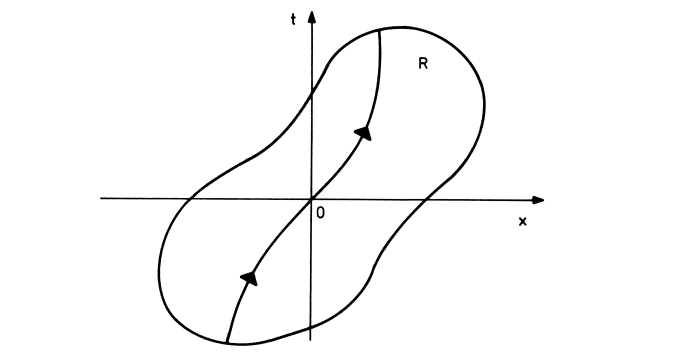
\includegraphics[width=0.9\textwidth]{img/latex2.png}

Fig. 5.19. La trayectoria espacio-temporal de una partícula puntual (o línea mundial de esta última) es un
proceso en el espacio-tiempo. A menos que haya realmente otras cosas en la región espacio-temporal
R, todos los puntos que no constituyan la línea mundial de la partícula son irrelevantes
y, por lo tanto, no merecen ser llamados «eventos».

\bigskip
colección de acontecimientos que ocurren en la cosa. Por eso nuestro estudio del
cambio fue precedido por un examen del concepto de cosa.
El dualismo de la metafísica del proceso es, por supuesto, la metafísica del ser. Una

versión de ello es el estructuralismo, actualmente en boga en Francia (cf. Uvi-
Strauss, 1958). Al igual que la metafísica tradicional oponía el ser al devenir
(o la cosa al proceso), e incluso ensalzaba uno de ellos a expensas del

otro, el estructuralismo tiende a oponer la estructura al cambio y a
separar la primera de las cosas. Al igual que los dinamistas extremos hablan de
acontecimientos sin cosas, los estructuralistas hablan de estructuras en sí mismas y
concentran su atención en la permanencia estructural en medio del flujo. Esto
también es erróneo: excepto en las matemáticas puras, donde hay estructuras
en sí mismas —por ejemplo, las álgebras booleanas—, toda estructura es la estructura de

alguna cosa (compleja): átomo, molécula, célula, órgano, organismo, comunidad,
 ecosistema o lo que sea. (Recordemos la definición 5.34 de la estructura
de una agregación de cosas). No decimos de un determinado objeto físico

que es un grupo de rotación, sino que una determinada propiedad del mismo (por ejemplo, la
energía) tiene simetría de rotación, o es invariante bajo rotaciones (miembros
del grupo de rotación). Del mismo modo, no decimos de una comunidad que es una
estructura social, sino que tiene tal estructura. Además, dada
la mutabilidad de todas las cosas, es poco probable que haya algo con una
estructura permanente. En resumen, la estructura es una propiedad, y una propiedad
mutable.

En conclusión, ni el procesismo ni el estructuralismo son alternativas viables
a nuestra metafísica de las cosas cambiantes. El devenir no es puro flujo,

 sino que consiste en el ser de las cosas en estados sucesivos, o en cosas sucesivas.
(Recuerde la Física de Aristóteles, libro III, capítulo 1, sección 1: «no existe tal
cosa como el movimiento por encima de las cosas»). Y las estructuras no solo son
volubles, sino que también carecen de existencia independiente: son estructuras de
las cosas, características de objetos concretos. En resumen, el cambio y la estructura son
características distintas pero entrelazadas de las cosas cambiantes dotadas de
alguna estructura u otra. Por lo tanto, los polos metafísicos tradicionales,
a saber, la metafísica del proceso y la metafísica del ser, tienen cada uno una pizca de
verdad y ambos son superados por nuestra ontología.
Llegamos al final de nuestro estudio del cambio en general. Hemos
formado los principales bloques de construcción para construir los conceptos de tiempo
y espacio. Una vez que estos estén disponibles, podremos dar una
explicación más detallada del cambio, en particular del cambio cualitativo,
que nos ocupará en el vol. 4, cap. 8. Pasamos entonces al estudio de la
extensión y la duración.
\noindent
  \end{justifying}
\end{justifying}